%!TEX root = thesis.tex

\chapter{Introduction}
\label{ch:intro}

\section{The Human-Computer Interface}


Human-Computer Interaction  (HCI) is slow. The information per minute rate is still low nowadays, and innovation is progressing slowly. Since the introduction of the mouse in the seventies almost no revolutionary new peripherals where introduced that aid the communication with a computer. (not completely true, Wii, (multi) touch screen).

\begin{figure}[htbp]
	\center{}
	\label{fig:mouse}
	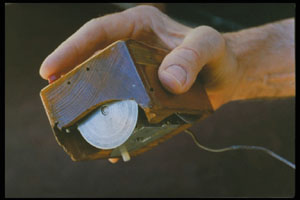
\includegraphics[width=0.3\linewidth]{figures/mouse.jpg}
	\caption{The first mouse}
\end{figure}

New and revolutionary ideas are required to create new peripherals that improve productivity, but are still intuitive and thus easy to learn to use. To get inspiration for improvement, one can look around and study already existing communication methods, for example the communication between humans. 

When two people are in a room and don't have a audio or visual limitation, they will probably communicate by speech. But there is much more going on than only producing and interpreting words. The intonation, speed and other small variations in the voice add a lot more information to the words. Also the facial expression and body language give more space for expression. Some people like to 'talk with their hands' while telling a story, something that adds more expression to the transmitted information.

\section{Sign Language}

A deaf person can't interpret spoken words, at least not by listening. He or she is highly depended on visual information. Sign languages have been created or invented to aid this visual communication. In these languages two elements have an important role, the face and the hands. These body parts give the most expressive power. The face because it is very good for expressing feelings and emotions, and the hands because they are very flexible and morphable. The hands are especially interesting because there are countless combinations of finger poses and orientations. 

Speech generation, speech recognition, facial expression recognition and sign language interpretation are all subject of extensive research at the moment.

Research has been done in automated sign language interpretation using computer vision\cite{Buehler2009}\cite{RichardBowden2004}. The problem with interpreting sign language is a very large vocabulary, segmentation of the different gestures and representing the gestures in a robust way.

\section{Goal and motivation}
\label{sec:goal}
The goal of this thesis is to describe the design, build and evaluation process of a system for hand pose recognition. The system needs to be fast and user friendly. Also the system should be able to run on current consumer hardware.

\begin{itemize}
	\item Real time performance (10+ fps)
	\item Normal consumer processing power
	\item Normal RGB camera (webcam)
	\item No gloves or skin mounted electromechanical sensors
	\item No calibration or initialization
	\item Minimal configuration/parameters
\end{itemize}
	

To realize these requirements some restrictions on the system's setting are required:
\begin{itemize}
	\item One person in the image
	\item Person is wearing clothing with long sleeves
	\item Good enough lightning conditions
	\item No skin like colors in the image.
\end{itemize}

The system can be used to aid HCI, but als add more feeling and detail, especially for real time interaction. Using hand poses for Computer aided music composing is interesting but challenging, since the realtime element plays an important role. Also, in a live performance setting, it is much more interesting to look at somebody using his body to interact with a machine than only click of a mouse.


\section{Solfege, The Curwen Hand symbols}

Any set of hand poses would do for this system, as long as the individual poses don't look to similar. But since the idea is to translate the interpreted hand poses into sound, it would be interesting to use a set of poses that has a already existing relationship to sound.

In Medieval music, the Guidonian hand was a mnemonic device used to assist singers in learning to sight sing. The idea of the Guidonian hand is that each portion of one hand represents a specific note within the hexachord system, which spans nearly three octaves. The other hand is used to point to the correct hand portion. \autoref{fig:guidonian} shows a hands with the tonal positions.

\begin{figure}[htbp]
	\center{}
	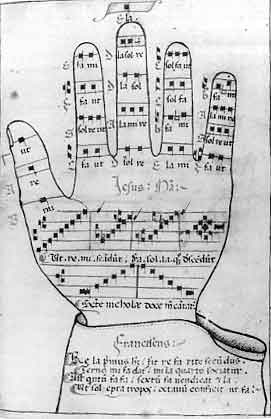
\includegraphics[width=0.3\linewidth]{figures/guidonian_hand.jpg}
	\label{fig:guidonian}
	\caption{Guidonian Hand}
\end{figure}

Despite this system has a large set of symbols - 22 to be exact - this system is not usable since the individual poses are very much alike. Discriminating between the different poses will probably be problematic.

A more recent method using hand poses in relation to music are the Curwen solfege hand signs\cite{choksy1999}. This method was introduced in the 19th century by John Curwen, who also is the founder of the famous tonic sol-fa. The tonic sol-fa is better known as \emph{'do re mi fa sol la ti'}.

\begin{figure}[htbp]
	\center{}
	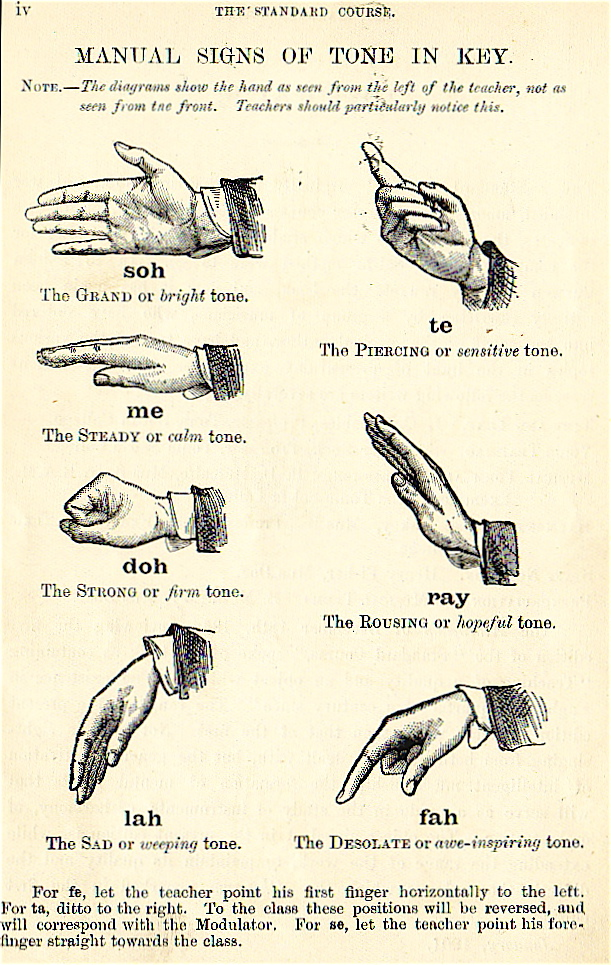
\includegraphics[width=0.6\linewidth]{figures/curwen.jpg}
	\label{fig:curwen}
	\caption{Depiction of Curwen's Solfege hand signs from 1904. This version includes the tonal tendencies and interesting titles for each tone.}
\end{figure}

\autoref{fig:curwen} is a scan from a teaching book from 1904 where the 6 tonal hand poses are shown. These 6 poses correspond to the 6 notes in the musical major scale. These hand poses are much more suitable for our system, since the individual hand symbols are distinct. Also the hand poses can be easily performed by both hands individually next to the body or in front of the body. \autoref{fig:curwennotes} shows the same hand symbols with the correspronding musical tones.

\begin{figure}[htbp]
	\center{}
	\subfloat{
		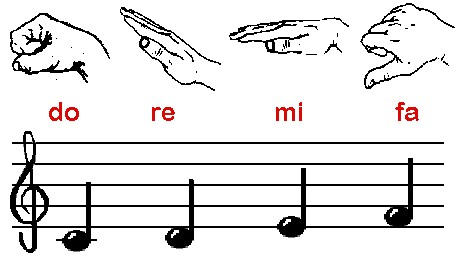
\includegraphics[width=0.45\linewidth]{figures/doremifa.jpg}
	}
	\hspace{0.03\linewidth}
	\subfloat{
		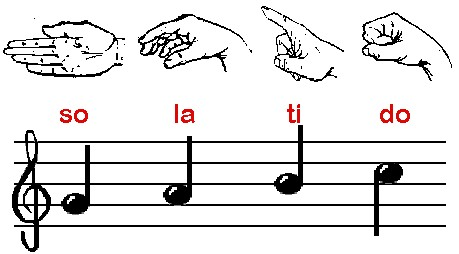
\includegraphics[width=0.45\linewidth]{figures/solatido.jpg}
	}
	\caption{The curwen hand symbols and the corresponding musical notes}
	\label{fig:curwennotes}
\end{figure}




\section{Related Work}
At the moment of writing this thesis Microsoft is finishing the development of a new commercial product called 'Kinect'. Kinect is claimed to provide full-body 3D motion capture. To accomplish this, Kinect uses a range camera, which interprets 3D scene information from a continuously-projected infrared pattern. For this setting a infrared projector and a range camera is required.

\begin{figure}[htbp]
	\center{}
	\label{fig:kinect}
	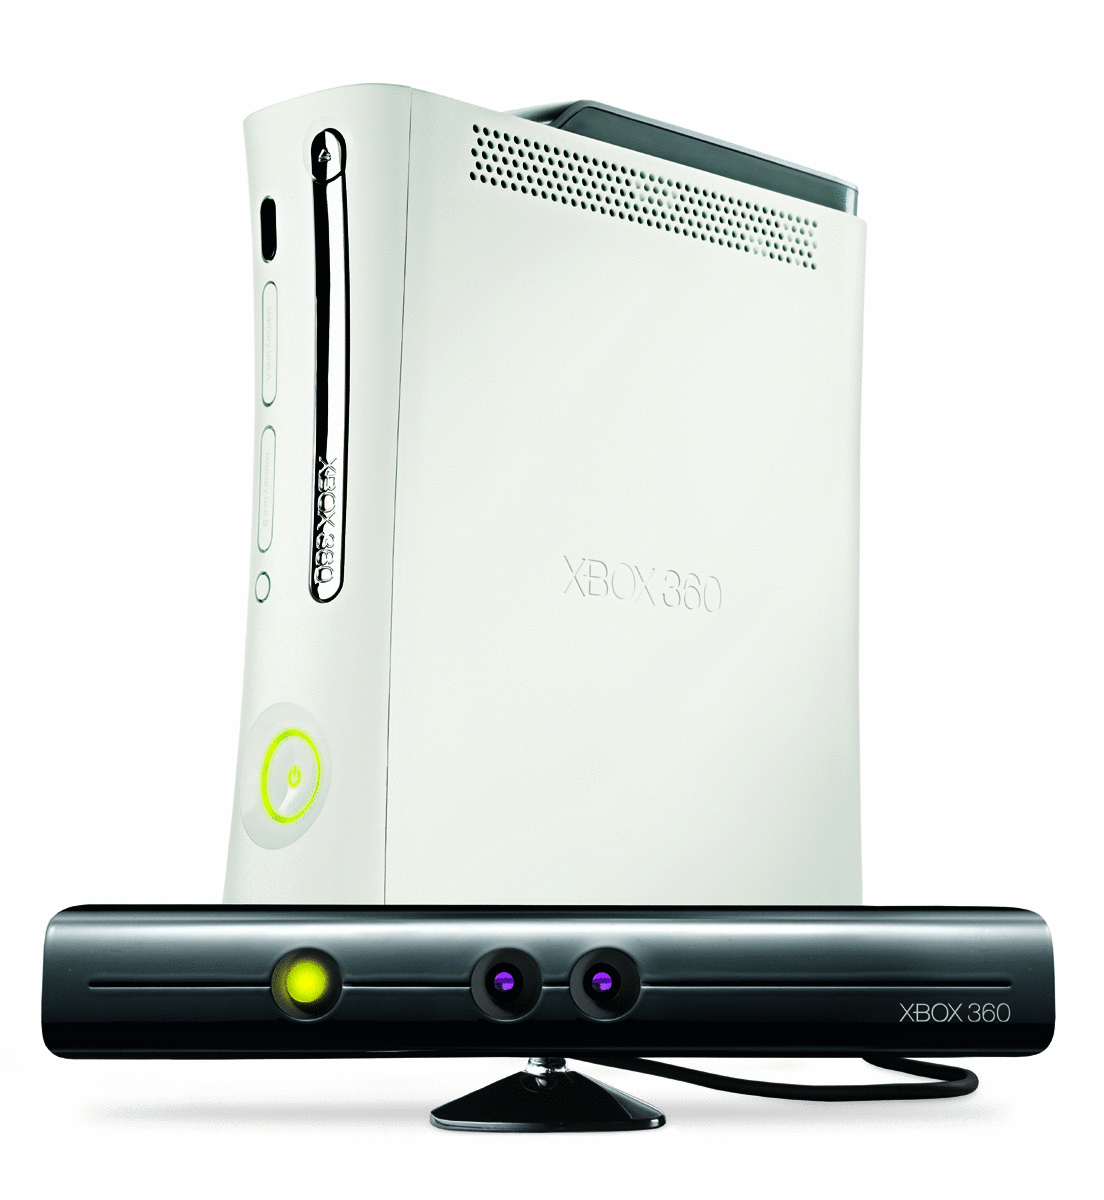
\includegraphics[width=0.3\linewidth]{figures/wave.jpg}
	\caption{Microsoft Kinect}
\end{figure}


An other interesting development is \cite{Wang2009} where a colored glove is used to perform full 3d hand pose estimation.

\begin{figure}[htbp]
	\center{}
	\label{fig:wang2009}
	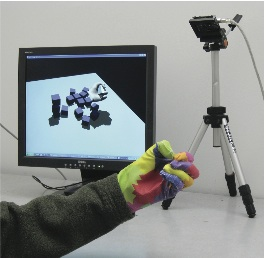
\includegraphics[width=0.3\linewidth]{figures/wang2009.jpg}
	\caption{3d hand pose estimation using a colored glove}
\end{figure}

An interesting overview paper is \cite{Erol2007}, which reviews the current state, possibilities and limitations of computer vision based hand pose and gesture recognition.


Similar research has been done \cite{Wang2007}. Here SIFT features are used to discriminate 3 different hand symbols. A performance of 95.6\% is claimed using a the 'sharing feature concept'.





others:

A PhD thesis exploring the hand as a input device: \cite{Sturman1992}

A very old paper using hand motion for segmentation: \cite{Cui1996}

Color based tracking a face for computer input \cite{Bradski1998}

Old paper using shadows to estimate 3d hand pose \cite{Segen1999}



